\documentclass[10pt,a4paper, titlepage]{report}

% Pacchetti...
% ----------------------------------------------------------------------------------------- %
\usepackage[T1]{fontenc}
\usepackage[utf8]{inputenc}
\usepackage[italian]{babel}
\usepackage{booktabs}
\usepackage{amsmath}
\usepackage{amsfonts}
\usepackage{amssymb}
\usepackage{listings}
\usepackage{xcolor}
\usepackage{graphicx}
\usepackage{sidecap}
\usepackage{float}
\usepackage{siunitx}
\usepackage{multirow}
\usepackage{hyperref}
\usepackage{bmpsize}
\usepackage{adjustbox}
\usepackage{footnote}


% Usato per personalizzare l'ambiente 'listings'...
% ----------------------------------------------------------------------------------------- %
\lstset{
language=C,
basicstyle=\small\ttfamily,			
keywordstyle=\color{blue},
commentstyle=\color{gray},			
stringstyle=\color{black},			
numbers=left,						
numberstyle=\tiny,					
stepnumber=1,						
breaklines=true						
}

% Usato per aggiugnere la numerazione alle sezioni di tipo 'subsubsection' e inserirle nell'indice...%
\setcounter{secnumdepth}{3}
\setcounter{tocdepth}{3}

% Frontespizio...
% ----------------------------------------------------------------------------------------- %
\title{Progetto del corso Ingegneria di Internet e del Web a.a. 2017-2018}
\author{Andrea Graziani - matricola 0189326}
\date{19 dicembre 2017}

% Inzio documento...
% ----------------------------------------------------------------------------------------- %
\begin{document}

\maketitle
\tableofcontents
\newpage

\chapter{Descrizione dell'applicazione}

L'applicazione di rete sviluppata, eseguibile su sistemi operativi basati su Linux, consente, attraverso un proprio protocollo applicativo, la comunicazione e la trasmissione \textit{affidabile} di dati tra host utilizzando, come protocollo di trasporto, UDP (\textit{User Datagram Protocol}). 

Nel corso di questa relazione descriveremo le caratteristiche del protocollo applicativo utilizzato nonché le modalità attraverso cui viene garantita la trasmissione affidabile dei dati.

\section{Architettura}

L'architettura dell'applicazione di rete è di tipo \textbf{client-server} dove un host chiamato \textit{server} è incaricato di soddisfare le richieste di servizio di molti altri host, detti \textit{client}.

Sappiamo che la maggior parte dei server che utilizzano il protocollo di trasporto UDP, come ad esempio i server DNS\footnote{Cfr. Andrew S. Tanenbaum \& David J. Wetherall - \textit{Reti di calcolatori 5/Ed}, Pearson, pp. 189}, è \textit{iterativa}\footnote{Cfr. Richard Stevens \& Bill Fenner \& Andrew M. Rudoff - \textit{UNIX Network Programming Volume 1, Third Edition: The Sockets Networking API}, Addison Wesley, Cap. 22.7}; in questo caso è sufficiente che il server attenda un messaggio di richiesta da parte di un client, quindi, dopo aver letto ed elaborato la richiesta ricevuta, spedisce un messaggio di risposta al client per poi attendere il successivo messaggio di richiesta. 

Tuttavia questo approccio, per quanto di semplice implementazione, non è adatta quando l'elaborazione della richiesta del client richiede "\textit{molto tempo}". Ad esempio, se arrivano due messaggi di richiesta entro 10 ms l'una dall'altra e il server impiega una media di 5 secondi per servire un client, il secondo client dovrà aspettare circa 10 secondi prima di ricevere una qualche risposta; qualora una richiesta fosse gestita immediatamente senza alcuna attesa, il secondo client attenderà, invece, circa 5 secondi. Da questo semplice esempio è facile capire che realizzando un'applicazione per il trasferimento di file, in cui spesso si richiede la trasmissione di molti pacchetti (centinaia o migliaia, a seconda delle dimensioni del file), i tempi di attesa possono diventare inaccettabili.

\begin{figure}
\centering
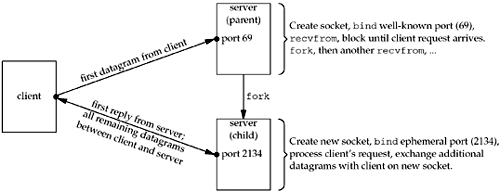
\includegraphics[width=\textwidth]{Concorrente}
\caption{Schema del funzionamento di un server UDP concorrente.}
\label{fig:Concorrente}
\end{figure}

Di conseguenza, data l'impraticabilità di un approccio iterativo, si è scelto di realizzare un'applicazione di rete di tipo \textbf{concorrente} di cui riportiamo uno schema in figura \ref{fig:Concorrente}. In un server UDP concorrente il compito di gestire e soddisfare le richieste ricevute dai client, in modo tale da permettere al processo server di poter continuare a ricevere nuove richieste, viene affidata ad un processo (o \textit{thread}) distinto da quello principale creandolo al momento oppure scegliendolo da un pool di processi precedentemente creati. Nei paragrafi seguenti analizzeremo nel dettaglio il funzionamento di un server UDP concorrente.


\subsection{Gestione delle richieste}
\subsubsection{Il processo server}\label{subsubsec:server}

Dopo aver aver stabilito la natura concorrente dell'architettura dell'applicazione sviluppata, esaminiamo ora alcuni aspetti implementativi del lato server dell'applicazione incominciando dalla gestione delle richieste.

Come è possibile osservare dalla porzione di codice raffigurante la funzione \texttt{start\_server} (implementata all'interno del file \texttt{server\_manager.c}) riportata in \textit{listing} \ref{code:serverStart}, l'attività svolta dal processo server principale è suddivisibile nelle seguenti fasi:

\begin{description}
\item[Inizializzazione socket ascolto] In questa fase, mediante l'esecuzione della funzione \texttt{\_\_server\_initialization} (anch'essa implementata all'interno del file \texttt{server\_manager.c}), avviene la procedura di inizializzazione di un \textit{socket di ascolto} su una porta \textit{nota}; ogni client intenzionato a trasmettere una richiesta al server dovrà inviare un opportuno messaggio di richiesta attraverso il suddetto socket.
\item[Caricamento metadati] Questa fase prevede il caricamento di una serie di informazioni utili a soddisfare richieste di tipo \texttt{list}; questo aspetto verrà approfondito nel paragrafo~\ref{sec:list-command}
\item[Fase di ascolto] Dopo aver allocato un'apposita area di memoria dove allocare il messaggio ricevuto dal client, il server (mediante la chiamata di sistema \texttt{recvfrom} di tipo \textit{bloccante}) rimane in attesa attendendo l'arrivo di un messaggio di richiesta sulla socket di ascolto precedentemente creata.
\item[Creazione del thread] Non appena viene ricevuto un nuovo messaggio di richiesta, viene creato un nuovo thread a cui affidare il compito di gestire e soddisfare la richiesta ricevuta. Successivamente il processo server ritorna in fase di ascolto.

\end{description}

\begin{lstlisting}[frame=lines, caption={Implementazione della funzione \texttt{start\_server}}, label={code:serverStart}]
void start_server() {

	ThreadArgument *ThreadArgument_obj;
	int received_bytes;

	/* Listener Socket file descriptor: Initialization server */
	int listener_socket_fd = __server_initialization(1);

	/* Preload metadata about shared files stored in application server directory */
	__metadata_preload();

	...

	while (1) {

		/* Preparing necessary data...  */
		/* ******************* */
		ThreadArgument_obj = calloc(1, sizeof(ThreadArgument));
		if (ThreadArgument_obj == NULL)
			exit_failure("calloc");

		ThreadArgument_obj->DataNetwork_obj.address_len = sizeof(ThreadArgument_obj->DataNetwork_obj.address);

		...

		/* Receiving request from client */
		/* ******************* */
		while (1) {

			errno = 0;
			received_bytes = recvfrom(listener_socket_fd, &ThreadArgument_obj->RequestPacket_obj, sizeof(RequestPacket), 0,
					(struct sockaddr *) &ThreadArgument_obj->DataNetwork_obj.address, &ThreadArgument_obj->DataNetwork_obj.address_len);

			...
		}
		...
		/* Launch thread */
		/* ******************* */
		thread_initialization(thread_job, (void **) ThreadArgument_obj);
	}
}
\end{lstlisting}

Questo approccio, per quanto semplice, presenta tuttavia un inconveniente. Il server UDP deve poter scambiare più di un pacchetto con il client per poter soddisfarne le richieste. Il problema è che l'unico numero di porta noto al client per poter comunicare con il server è, sfortunatamente, la stessa porta utilizzata da quest'ultimo per ricevere nuove richieste. Dopo che il client ha inviato un messaggio di richiesta attraverso la porta di ascolto, come fa dunque il server a distinguere tra pacchetti successivi provenienti da quel client e nuove richieste? 

La soluzione è quella di affidare ai thread incaricati di soddisfare le richieste ricevute anche il compito di creare un'apposita socket di supporto eseguendo il binding su una porta effimera e utilizzando quel socket per inviare e ricevere i successivi messaggi con un client. Ciò ovviamente richiede che il client in questione guardi il numero di porta della prima risposta del server e invii i pacchetti successivi a quella porta. Tutto ciò consente al server principale di continuare a gestire altre richieste proveniente da altri client. 

\subsubsection{Il processo client}

In accordo alle specifiche di progetto, ogni processo client, senza alcuna operazione di autenticazione preliminare, deve essere in grado di:
\begin{itemize}
\item Visualizzare tutti i file disponibili sul server;
\item Scaricare file dal server;
\item Caricare file sul server;
\end{itemize}
L'esecuzione  delle suddette operazioni è possibile previo l'invio da parte del client di un apposito \textit{messaggio di richiesta} al processo server.

Da un punto di vista implementativo, per poter inoltrare una qualsiasi richiesta, il processo client fa uso di due strutture dati fondamentali:

\begin{description}
\item[\texttt{DataNetwork}] Essa rappresenta tecnicamente un contenitore per tutte le informazioni necessarie per comunicare con un host, ovvaro indirizzo IP e numero di porta. Tale struttura, utilizzata sia dal processo client che da quello server e di cui riportiamo il codice in \textit{listing} \ref{code:DataNetwork}, è composta da:
\begin{enumerate}
\item Un campo ospitante il \textit{file descriptor} di una socket.
\item Un campo contente una struttura di tipo \texttt{sockaddr\_in} all'interno della quale sono contenute le informazioni necessarie per comunicare con un host.
\item Un campo utilizzato per ospitare un quantità di tipo \texttt{socklen\_t} che specifica la lunghezza della struttura \texttt{sockaddr\_in} precedente.
\end{enumerate}

\begin{lstlisting}[frame=lines, caption={Implementazione della struttura \texttt{DataNetwork}}, label={code:DataNetwork}]
typedef struct data_network {

	/* Socket file descriptor */
	int socket_fd;
	/* Internet socket address */
	struct sockaddr_in address;
	/* Internet socket address length */
	socklen_t address_len;

} DataNetwork;
\end{lstlisting}


\item[\texttt{RequestPacket}] Questa struttura modella un \textit{messaggio di richiesta} ed è composta da:
\begin{enumerate}
\item Un campo di 35 byte utilizzato per ospitare una speciale struttura dati, denominata \texttt{Settings}, utilizzata per ospitare una serie di parametri trasmissivi tra cui la dimensione della finestra di spedizione, durata di timeout e probabilità di perdita dei messaggi. Approfondiremo in seguito i dettagli relativi alle impostazioni.
\item Un campo di 1 byte utilizzato per specificare il tipo di richiesta (\textit{list}, \textit{put} e \textit{get}).
\item Un campo di dimensione eventualmente nulla inferiore ai 255 byte utilizzato per specificare un eventuale parametro o informazione aggiuntiva; per esempio, se il client trasmettesse un messaggio di tipo \textit{get}, il suddetto campo conterrebbe il nome di un file.
\end{enumerate}
\end{description}

\begin{lstlisting}[frame=lines, caption={Implementazione della struttura \texttt{RequestPacket}}, label={code:RequestPacket}]
typedef struct request_client_packet {

	Settings client_setting;
	char request_type;
	char request_type_argument[NAME_MAX];

} RequestPacket;
\end{lstlisting}

Per inviare un messaggio di richiesta il processo client non fa altro che inizializzare opportunamente una struttura di tipo \texttt{RequestPacket} inviandola al server servendosi delle informazioni contenute all'interno della struttura di tipo \texttt{DataNetwork} tra cui l'indirizzo IP, specificato dall'utente, e il numero della porta di ascolto sul server nota a priori, per poi attendere una risposta da parte del server. Qualora non si ricevesse alcuna risposta, il processo client deve provvedere a inoltrare nuovamente la richiesta.

Nel paragrafo precedente abbiamo stabilito che il client, conoscendo esclusivamente il numero della porta di ascolto, non può sapere da quale porta verranno scambiati i successivi messaggi con il server; pertanto il client dovrà guardare il numero di porta della prima risposta del server e, aggiornando opportunamente i valori dei campi contenuti nella struttura \texttt{DataNetwork}, inviare i pacchetti successivi a quella porta. Questa operazione molto delicata viene eseguita attraverso la funzione \texttt{\_\_receive\_datagram} definita all'interno del file \texttt{data\_transmission.c} di cui ne riportiamo il codice in \textit{listing} \ref{code:receiveDatagram}. Dopo la ricezione della prima risposta da parte del server, verrà aggiornato il contenuto della struttura \texttt{DataNetwork} consentendo al client non solo di poter scambiare altri messaggi ma anche di ignorare tutti quei pacchetti non provenienti dal processo server con cui interagisce; inoltre permette a quest'ultimo di ignorare tutti i pacchetti provenienti da altri client. Quest'ultima operazione è resa possibile mediante un semplice confronto dell'indirizzo IP e del numero di porta del messaggio ricevuto con le informazioni contenute all'interno della struttura da \texttt{DataNetwork}. 

\begin{lstlisting}[frame=lines, caption={Implementazione della funzione \_\_receive\_datagram}, label={code:receiveDatagram}]
int __receive_datagram(DataNetwork *DataNetwork_obj, void *buffer, size_t buffer_size, char *check_replay) {

	int bytes_received;

	...
	struct sockaddr *preply_addr = malloc(DataNetwork_obj->address_len);
	if (preply_addr == NULL)
		exit_failure("malloc");

	do {
		/* Receiving data in 'check replay' mode */
		/* ******************* */
		bytes_received = recvfrom(DataNetwork_obj->socket_fd, buffer, buffer_size, 0, preply_addr, &DataNetwork_obj->address_len);

		/* Checking error */
		if (bytes_received == -1) {
			if (errno == EINTR) {

				...

				/* Free memory */
				free(preply_addr);

				return -1;
			} else
				exit_failure("recvfrom_wc");
		}

		if (check_replay == NULL || *check_replay == CHECK_REPLAY) {

			/* Check reply */
			/* ******************* */
			if (memcmp((struct sockaddr*) &(DataNetwork_obj->address), preply_addr, DataNetwork_obj->address_len) != 0) {
				...
				continue;
			}

		} else {

			memcpy(&DataNetwork_obj->address, preply_addr, sizeof(*preply_addr));

			/* Check replay... */
			*check_replay = CHECK_REPLAY;
		}
	} while (0);

	/* Free memory */
	free(preply_addr);

	...

	return bytes_received;
}
\end{lstlisting}

\newpage
\section{Implementazione del servizio di trasmissione affidabile}

In questo capitolo descriveremo come è stato implementato un servizio di trasmissione affidabile utilizzando un protocollo di trasporto come UDP che offra un servizio di comunicazione di tipo \textit{best effort}\footnote{Cfr. Andrew S. Tanenbaum \& David J. Wetherall - \textit{Reti di calcolatori 5/Ed}, Pearson, pp. 179}, ovvero non affidabile.


\subsection{I messaggi di controllo}

Incominciamo con alcune constatazioni: 

\begin{itemize}
\item Dato che mittente e destinatario sono generalmente in esecuzione su sistemi periferici diversi, magari separati da migliaia di chilometri, l 'unico modo che ha il mittente per sapere se un pacchetto sia stato ricevuto correttamente o meno consiste nel \textit{feedback esplicito} del destinatario.
\item Dovendo rispettare le specifiche di progetto, l'applicazione deve simulare a livello applicativo un protocollo a \textbf{ripetizione selettiva} (o semplicemente SR, \textit{selective-repeat protocol}). Il protocollo SR ci consente di per evitare una serie di ritrasmissioni non necessarie in quanto il mittente deve ritrasmette solo quei pacchetti su cui esistono sospetti di errore, ossia smarrimento o alterazione, rilevati in base alla mancata o ritardata ricezione del riscontro di un pacchetto.

\end{itemize}

Queste due considerazioni costringono pertanto il destinatario a mandare riscontri specifici per i pacchetti ricevuti in modo corretto; questi riscontri costituiscono i cosiddetti \textit{messaggi di controllo}.

Da un punto di vista implementativo, per modellare i messaggi di controllo ci si è serviti di un'apposita struttura denominata \texttt{ControlDatagram} di cui riportiamo il codice in \textit{listing} \ref{code:ControlDatagram}. I messaggi di controllo vengono utilizzati per:

\begin{enumerate}
\item Inviare al mittente un riscontro (detto anche \textit{acknowledgement}, quest'ultimo abbreviato spesso con l'acronimo ACK) per i pacchetti ricevuti in modo corretto.
\item Gestire le procedure di instaurazione e chiusura delle connessioni.
\end{enumerate}

Una struttura di tipo \texttt{ControlDatagram} è composta dai seguenti campi:
\begin{enumerate}
\item Un campo di un byte utilizzato per specificare il \textit{tipo} di messaggio di controllo. I tipi utilizzati sono:
\begin{description}
\item[\texttt{REQ}] È usato per instaurare un connessione con un altro host; benché molto diverso, esso corrisponde al segmento \texttt{SYN} usato nel protocollo di trasporto TCP\footnote{Cfr. \textit{ivi}, pp. 239}.
\item[\texttt{REQ\_ACK}] È usato per rispondere ad una richiesta di connessione in seguito alla ricezione di un messaggio di tipo \texttt{REQ}; corrisponde al segmento \texttt{SYNACK} usato in TCP\footnote{Cfr. \textit{ibid.}}.
\item[\texttt{FIN}] Viene utilizzato per terminare una trasmissione e incominciare la procedura di chiusura della connessione; corrisponde al segmento \texttt{FIN} usato in TCP\footnote{Cfr. \textit{ibid.}}.
\item[\texttt{FIN\_ACK}] Viene utilizzato per confermare la terminazione di una trasmissione. 
\item[\texttt{CLS}] Viene utilizzato per terminare una connessione. 
\item[\texttt{ACK}] Viene utilizzato per indicare un messaggio di riscontro.
\end{description}

\item Un campo di un byte utilizzato per ospitare il \textit{numero di sequenza} di un pacchetto; tale campo è utilizzato esclusivamente quando il messaggio di controllo in questione rappresenta un ACK, in caso contrario la dimensione del campo è nulla.
\end{enumerate}

\begin{lstlisting}[frame=lines, caption={Implementazione della struttura \texttt{ControlDatagram}}, label={code:ControlDatagram}]
typedef struct control_datagram {
	char type;
	char n;
} ControlDatagram;
\end{lstlisting}

\subsection{Gestione delle ritrasmissioni}\label{subsec:ritrasmissioni}

Riuscire a rilevare e a gestire lo \textit{smarrimento} dei pacchetti, un evento non raro sulle odierne reti di calcolatori, e decidere cosa fare quando ciò avviene rappresenta il problema più importante e complesso. La soluzione a questo problema è tuttavia molto semplice: se dopo la trasmissione di un certo pacchetto il mittente non ricevesse alcun riscontro da parte del destinatario dopo un certo lasso di tempo, quest'ultimo deve provvedere a ritrasmettere il pacchetto smarrito. 

Implementare un meccanismo di ritrasmissione basato sul tempo richiede l'utilizzo di un \textit{timer} capace di segnalare al mittente l'avvenuta scadenza di un dato lasso di tempo e che il mittente sia in grado di:

\begin{enumerate}
\item Inizializzare un timer ogni volta che invia un pacchetto.
\item Rispondere adeguatamente all'interrupt generato dal timer in caso di timeout procedendo quindi alla ritrasmissione del pacchetto smarrito e reinizializzare il timer.
\item Disabilitare il timer quando il mittente riceve un riscontro positivo da parte del destinatario.
\end{enumerate}

Questo approccio introduce, tuttavia, la presenza di pacchetti duplicati nel canale di trasmissione. Dal momento che il destinatario non può sapere a priori se un pacchetto in arrivo contenga dati nuovi o rappresenti una ritrasmissione, è necessario utilizzare dei \textit{numeri di sequenza}: al destinatario sarà sufficiente controllare questo numero per sapere se il pacchetto si tratta di una ritrasmissione o meno. Inoltre, dal momento che l'applicazione simula il comportamento di un protocollo a ripetizione selettiva, sarà necessario  associare ad ogni pacchetto trasmesso un timer dedicato. 

\subsubsection{Calcolo dell'intervallo di timeout}\label{subsubsec:calc-timeout}

\begin{figure}
\centering
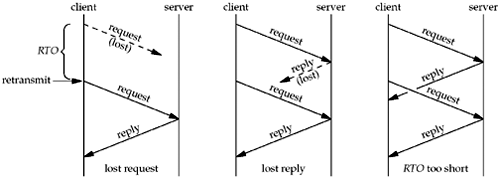
\includegraphics[width=\textwidth]{Timeout}
\caption{Possibili scenari che si possono verificare dopo un timeout}
\label{fig:Timeout}
\end{figure}

Occupiamoci ora di una questione cruciale: la lunghezza dell'intervallo di timeout. Ovviamente l'intervallo di timeout dovrebbe essere più grande del tempo di andata e ritorno del segnale sulla connessione per evitare timeout prematuri evitando così ritrasmissioni inutili. 
Per calcolare l'intervallo di timeout si usato lo stesso algoritmo utilizzato nel protocollo TCP. L'applicazione misura una quantità di tempo detta RTT (\textit{Round Trip Time}); quest'ultima rappresenta la quantità di tempo che intercorre tra l'istante di invio del segmento e quello di ricezione del relativo ACK. Tuttavia, in base alla congestione nei router e al diverso carico sui sistemi periferici durante la trasmissione, i campioni di RTT calcolati possono variare da pacchetto a pacchetto, perciò si preferisce calcolare una media dei valori di RTT: tale quantità, che chiameremo $EstimatedRTT$, si calcola con la seguente formula:

\begin{equation}
EstimatedRTT = (1 - \alpha) \times EstimatedRTT + \alpha \times RTT
\end{equation}

Dove $\alpha = 1/8$. Si noti che $EstimatedRTT$ è una media ponderata dei valori RTT: tale media, meglio conosciuta in statistica come \textbf{media mobile esponenziale ponderata} (EWMA, \textit{expo­nential weighted moving average}), attribuisce maggiore importanza ai campioni recenti rispetto a quelli vecchi in modo tale da riflettere meglio la congestione attuale della rete. Tuttavia, oltre a calcolare la media dei valori di RTT, è anche importante possedere anche la misura della variabilità dei RTT calcolati. Tale quantità verrà chiamata $DevRTT$ ed è calcolabile come segue:

\begin{equation}
DevRTT = (1 - \beta) \times DevRTT + \beta \times \mid RTT - EstimatedRTT \mid
\end{equation}

Come già detto, l 'intervallo di timeout non può essere inferiore a quello di $EstimatedRTT$, altrimenti verrebbero inviate ritrasmissioni non necessarie. Ma l 'intervallo stesso non dovrebbe essere molto maggiore di $EstimatedRTT$, altrimenti avremo gravi ritardi sul trasferimento dei dati. È pertanto auspicabile impostare il timeout a $EstimatedRTT$ più un certo margine che dovrebbe essere grande quando c'è molta fluttuazione nei valori di RTT e piccolo in caso contrario. Qui entra in gioco il valore di $DevRTT$. Tutti questi aspetti vengono presi in considerazione dalla seguente equazione:

\begin{equation}
RTO = EstimatedRTT + 4 \times DevRTT
\end{equation}

Da un punto di vista implementativo, tutte le informazioni riguardante la durata dell'intervallo di timeout (indicata con l'acronimo RTO, \textit{Recovery Time Objective}), la media dei valori di RTT e la loro varianza sono contenute all'interno di una speciale struttura denominata \texttt{TimeInfo} definita all'interno del file \texttt{time\_management.h} di cui riportiamo il codice in \textit{listing} \ref{code:time_info}.

\begin{lstlisting}[frame=lines, caption={Implementazione della struttura \texttt{time\_info}}, label={code:time_info}]
typedef struct time_info {

	/* Current 'Recovery Time Objective' (RTO) to use */
	struct timespec RTO;

	/* Weighted average of RTT values */
	struct timespec Estimated_RTT;
	/* Variance */
	struct timespec Dev_RTT;

} TimeInfo;
\end{lstlisting}

L'algoritmo descritto in precedenza per il calcolo degli intervalli di timeout è implementato all'interno della funzione \texttt{TimeInfo\_calc\_time} definita all'interno del file \texttt{time\_management.c} di cui ne riportiamo il codice in \textit{listing} \ref{code:time_info_calc}. 

\begin{lstlisting}[frame=lines, caption={Implementazione della funzione \texttt{TimeInfo\_calc\_time}}, label={code:time_info_calc}]
/*
 * Updates RTT estimators and calculates new RTO.
 *
 * @param *input -> It represents a 'TimeInfo' object.
 * @param *sending_time -> It represents a 'timespec' object.
 * @param *receiving_time -> It represents a 'timespec' object.
 */
void TimeInfo_calc_time(TimeInfo *input, struct timespec *sending_time, struct timespec *receiving_time) {

	const float alpha = 0.125;
	const float beta = 0.25;

	struct timespec RTT;

	/* Calculation */
	/* =============== */

	/* Calculate 'Round Trip Time' */
	RTT.tv_sec = receiving_time->tv_sec - sending_time->tv_sec;
	RTT.tv_nsec = receiving_time->tv_nsec - sending_time->tv_nsec;

	/* Calculate weighted average of RTT values */
	input->Estimated_RTT.tv_sec = (1.0 - alpha) * input->Estimated_RTT.tv_sec + alpha * RTT.tv_sec;
	input->Estimated_RTT.tv_nsec = (1.0 - alpha) * input->Estimated_RTT.tv_nsec + alpha * RTT.tv_nsec;

	/* Calculate variance */
	input->Dev_RTT.tv_sec = (1.0 - beta) * input->Dev_RTT.tv_sec + beta * abs(RTT.tv_sec - input->Estimated_RTT.tv_sec);
	input->Dev_RTT.tv_nsec = (1.0 - beta) * input->Dev_RTT.tv_nsec + beta * abs(RTT.tv_nsec - input->Estimated_RTT.tv_nsec);

	/* Calculate RTO */
	input->RTO.tv_sec = input->Estimated_RTT.tv_sec + (4.0 * input->Dev_RTT.tv_sec);
	input->RTO.tv_nsec = input->Estimated_RTT.tv_nsec + (4.0 * input->Dev_RTT.tv_nsec);

	/* Converting nanosec to sec */
	/* =============== */
	__timespec_converting_from_ns_to_s(&input->RTO);
	__timespec_converting_from_ns_to_s(&input->Estimated_RTT);
	__timespec_converting_from_ns_to_s(&input->Dev_RTT);

	/* Checking if RTO is within the permitted limits... */
	/* =============== */
	__timespec_checking_limit(&input->RTO);
}
\end{lstlisting}

Per concludere è opportuno precisare che le strutture \texttt{TimeInfo} vanno inizializzate mediante la funzione \texttt{TimeInfo\_init} definita nel file \texttt{time\_management.c} prima di essere utilizzate; questa operazione è necessaria sia per impostare un intervallo di timeout iniziale, che in accordo alle [RFC 6298]\footnote{Cfr. Andrew S. Tanenbaum \& David J. Wetherall - \textit{Reti di calcolatori 5/Ed}, Pearson, pp. 228} deve essere impostato ad un secondo, sia per impostare eventualmente un intervallo di timeout stabilito dall'utente 

\subsubsection{I Timer}

Dovendo simulare il comportamento di un protocollo di trasmissione selettiva, ogni pacchetto trasmesso dal mittente deve essere associato ad un proprio timer logico. In particolare, i timer associato ad uno specifico pacchetto deve essere attivato all'atto della sua trasmissione. Dopo la trasmissione di un pacchetto possono verificarsi due eventi:

\begin{enumerate}
\item Il mittente riceve un riscontro da parte del destinatario; il timer viene pertanto disattivato. 
\item Il mittente non riceve alcun riscontro da parte del destinatario fino allo scadere dell'intervallo di timeout; il timer genera quindi un interrupt in seguito alla quale il mittente provvederà a ritrasmettere il pacchetto associato a quel timer.
\end{enumerate}

Da un punto di vista implementativo, per allocare e assegnare un timer logico a ciascun pacchetto da trasmettere, si è usato un'apposita struttura denominata \texttt{DatagramTimer} definita all'interno del file \texttt{time\_management.h} e di cui riportiamo il codice in \textit{listing} \ref{code:DatagramTimer}. Questa struttura comprende:

\begin{itemize}
\item Un puntatore al pacchetto associato al timer.
\item Un puntatore ad un oggetto di tipo \texttt{DataNetwork}.
\item Un puntatore denominato \texttt{abort\_trasmission\_ptr} utilizzato per interrompere il processo di trasmissione qualora venga superato il limite massimo di ritrasmissioni consentite per quel pacchetto.
\item Un campo utilizzato per specificare il tipo di pacchetto associato al timer e distinguere perciò i pacchetti ordinari contenti dati dai messaggi di controllo.
\item Un oggetto di tipo \texttt{timer\_t} rappresentante un timer UNIX\footnote{Cfr. Michael Kerrisk - \textit{The Linux Programming Interface}, No Starch Press, pp. 495-496}.
\item Il numero di ritrasmissione effettuate per un dato pacchetto.
\item Un oggetto di tipo \texttt{itimerspec}\footnote{Cfr. \textit{ivi}, pp. 480} usato per rappresentare la durata l'intervallo di timeout.
\item Due oggetti di tipo \texttt{timespec} usati per indicare l'istante di invio del pacchetto e ricezione del relativo riscontro.
\end{itemize}

\begin{lstlisting}[frame=lines, caption={Implementazione della struttura \texttt{DatagramTimer}}, label={code:DatagramTimer}]
typedef struct datagram_timer {

	void *Datagram_ptr;
	DataNetwork *DataNetwork_ptr;
	char *abort_trasmission_ptr;

	char datagram_type;
	timer_t timer;
	char times_retrasmitted;
	struct itimerspec timervals;
	struct timespec sending_time;
	struct timespec receiving_time;
	
} DatagramTimer;
\end{lstlisting}

\subsubsection{Configurazione e gestione dei timer}

Ora che abbiamo definito le strutture di tipo \texttt{DatagramTimer}, descriviamo come possono essere utilizzate. Innanzitutto, per poter usare un timer e associarlo ad uno specifico pacchetto, è necessario eseguire una procedura di inizializzazione attraverso una funzione denominata \texttt{DatagramTimer\_init} e implementata nel file \texttt{time\_management.c} di cui riportiamo il codice in \textit{listing} \ref{code:DatagramTimerInit}.

Operativamente, l'inizializzazione di un oggetto di tipo \texttt{DatagramTimer} si divide nelle seguenti fasi:

\begin{description}
\item[Associazione del pacchetto] Popolando opportunamente i campi della struttura \texttt{DatagramTimer}, si specifica il pacchetto associato al timer in questione. In questa fase viene popolato anche il puntatore alla struttura di tipo \texttt{DataNetwork} necessario per ritrasmettere il pacchetto in caso di timeout.
\item[Configurazione handler] In questa fase viene dichiarata la procedura da seguire in caso di timeout; operativamente viene specificato un apposito handler attraverso l'uso della chiamata di sistema \texttt{sigaction}.
\item[Configurazione della struttura \texttt{sigevent}] Questa fase è necessaria per specificare come l'applicazione debba essere avvisata dell'avvenuto timeout; ciò viene effettuato attraverso la configurazione di una speciale struttura dati di tipo \texttt{sigevent}\footnote{Cfr. \textit{ivi}, pp. 496}. In particolare il metodo di notifica scelto è di tipo  \texttt{SIGEV\_THREAD\_ID}: in accordo alle specifiche delle API POSIX, scegliendo il suddetto metodo di notifica, in seguito al verificarsi di un timeout, il timer invia un segnale a quel thread il cui identificatore coincide con il valore specificato in \texttt{sigev\_un.\_tid}. Popolando opportunamente il campo \texttt{sigev\_value.sival\_ptr} con un puntatore ad una struttura di tipo \texttt{DatagramTimer}, l'handler incaricato di gestire l'avvenuto timeout potrò accedere al pacchetto associato al timer appena scaduto.
\item[Creazione del timer] In questa fase avviene semplicemente la creazione del timer attraverso la chiamata di sistema \texttt{timer\_create()}\footnote{Cfr. \textit{ivi}, pp. 495} usata compatibilmente alle specifiche delle API POSIX. 
\end{description}

\begin{lstlisting}[frame=lines, caption={Implementazione della funzione \texttt{DatagramTimer\_init}}, label={code:DatagramTimerInit}]
void DatagramTimer_init(DatagramTimer *DatagramTimer_obj, void **Datagram_ptr, DataNetwork **DataNetwork_ptr, char *abort_trasmission_ptr,
		char datagram_type, void (*handler)(int, siginfo_t*, void*)) {

	struct sigevent sev;
	struct sigaction sa;

	/* Configuration 'DatagramTimer' */
	/* =============== */
	if (DataNetwork_ptr != NULL)
		DatagramTimer_obj->DataNetwork_ptr = *DataNetwork_ptr;
	if (Datagram_ptr != NULL)
		DatagramTimer_obj->Datagram_ptr = *Datagram_ptr;

	DatagramTimer_obj->abort_trasmission_ptr = abort_trasmission_ptr;
	DatagramTimer_obj->datagram_type = datagram_type;

	/* Establish handler for notification signal */
	/* =============== */
	sa.sa_flags = SA_SIGINFO;
	sa.sa_sigaction = handler;
	sigemptyset(&sa.sa_mask);
	sigaddset(&sa.sa_mask, SIGRTMAX);
	if (sigaction(SIGRTMAX, &sa, NULL) == -1)
		exit_failure("sigaction");

	/* Configuration structure to transport application-defined values with signals. */
	/* =============== */
	sev.sigev_notify = SIGEV_THREAD_ID;
	sev._sigev_un._tid = syscall(SYS_gettid);
	sev.sigev_signo = SIGRTMAX;
	sev.sigev_value.sival_ptr = DatagramTimer_obj;

	/* Create new per-process timer using CLOCK_ID. */
	/* =============== */
	if (timer_create(CLOCK_REALTIME, &sev, &DatagramTimer_obj->timer) == -1)
		exit_failure("timer_create");
}
\end{lstlisting}

Una volta inizializzato l'oggetto \texttt{DatagramTimer} è possibile avviare un timer attraverso la chiamata di sistema \texttt{timer\_settime()}\footnote{Cfr. \textit{ivi}, pp. 498}; la durata dell'intervallo di timeout può essere aggiornata attraverso i valori calcolati e contenuti all'interno della struttura \texttt{TimeInfo}. La disattivazione di un timer in seguito alla ricezione di un riscontro positivo avviene utilizzando la chiamata di sistema \texttt{timer\_settime()} specificando un intervallo di timeout nullo\footnote{Cfr. \textit{ibid}}.
Una volta completato il processo di trasferimento dei dati, tutti i timer precedentemente allocati possono essere rimossi mediante la chiamata di sistema \texttt{timer\_delete()}\footnote{Cfr. \textit{ivi}, pp. 499}. 

\newpage

\section{Gestione della trasmissione}\label{sub:gestione-della-trasmissione}

Descriveremo ora le modalità attraverso cui un processo client e un processo server possano effettivamente scambiarsi dati. Il protocollo applicativo realizzato è principalmente descritto all'interno del \texttt{data\_transmission.c} dove sono presenti diverse funzioni tra cui:

\begin{itemize}
\item \texttt{receiving\_data\_selective\_repeat}
\item \texttt{sending\_data\_selective\_repeat}
\end{itemize}

La prima funzione descrive il comportamento adottato dal destinatario mentre la seconda quello del mittente. Analizzando le suddette funzioni è possibile comprendere che qualsiasi operazione di trasferimento dati richiede le seguenti operazioni: 

\begin{description}
\item[Inizializzazione della trasmissione] Durante questa fase devono essere allocate e inizializzate tutte le strutture dati necessarie per eseguire la trasmissione tra cui:
\begin{itemize}
\item Un \textit{buffer di ricezione} (lato client) e un \textit{buffer di invio} (lato server) entrami di dimensione $N$. La relazione ottimale\footnote{Cfr. Achille Pattavina - \textit{Reti di telecomunicazione, Networking e Internet, Seconda edizione}, McGraw-Hill, pp. 114} tra la dimensione dei buffer $N$ e la dimensione dell'apertura della finestra di spedizione $W$ è:

\begin{equation}
N = 2W
\end{equation}

\item Un \textit{buffer di supporto} di dimensione $N$ utilizzato dal server per ospitare oggetti di tipo \texttt{DatagramTimer}; quest'ultimi sono necessari per eseguire l'associazione tra i timer e i corrispondenti pacchetti contenuti nel buffer di invio. Tale associazione avviene nel modo seguente: sia $A$ il buffer di invio e sia $B$ il buffer di supporto contenente i timer; il pacchetto $A[i]$ sarà associato al timer $B[i]$ con $0 \leq i \leq N - 1$. In altri termini il pacchetto $k$-esimo contenuto nel buffer di invio verrà associato al $k$-esimo oggetto \texttt{DatagramTimer} contenuto nel buffer di supporto. Nel codice sorgente questo buffer è denominato \texttt{DatagramTimer\_buffer}.

\item Un oggetto di tipo \texttt{TimeInfo} che verrà utilizzato per ospitare le informazioni necessarie per eseguire il calcolo e l'aggiornamento della durata dell'intervallo di timeout in base alle condizioni della rete.

\item Un oggetto di tipo \texttt{NetworkStatistics} che verrà utilizzato per elaborare una serie di informazioni utili all'analisi delle prestazioni del protocollo tra cui: il numero totale di pacchetti inviati; il numero di timeout che si sono verificati durante la trasmissione; l'istante di avvio e di chiusura della trasmissione e altro ancora.

\item Una serie di variabili di controllo necessarie a gestire la connessione. Invitiamo ad analizzare il codice sorgente per una descrizione dettagliata.
\end{itemize}

\item[Instaurazione della trasmissione] Questa fase, similmente a quanto avviene in TCP, prevede che mittente invii per primo uno messaggio di controllo di tipo \texttt{REQ}; alla ricezione di quest'ultimo, il destinatario risponde con un messaggio di controllo di tipo \texttt{REQ\_ACK}. Ricordiamo che i primi due messaggi non trasportano payload, ossia non hanno dati a livello applicativo. In seguito alla ricezione del messaggio \texttt{REQ\_ACK}, il mittente potrà finalmente inviare il primo pacchetto ordinario contenente dati di interesse. Dato che i due host si scambiano tre pacchetti, questa procedura che instaura una connessione viene detta \textbf{handshake a tre vie} (\textit{three-way handshake})\footnote{Cfr. Andrew S. Tanenbaum \& David J. Wetherall - \textit{Reti di calcolatori 5/Ed}, Pearson, pp. 239}.
 
\item[Trasmissione dati] In questa fase avviene la trasmissione dati vera e propria. Per motivi di spazio analizzeremo nel dettaglio solo il comportamento del mittente (il comportamento del destinatario è perfettamente analogo a quello previsto dal protocollo SR) il quale svolge le seguenti operazioni: 

\begin{description}
\item[Incapsulamento dati] In questa fase il mittente legge dal file system i dati da inviare al mittente e li incapsula all'interno di un pacchetto ordinario rappresentato da una struttura di tipo \texttt{Datagram}. Quest'ultimo verrà ovviamente inserito nel buffer di invio e automaticamente associato ad un timer logico. 
\item[Invio] In questa fase il mittente invia al destinatario il pacchetto precedentemente creato attivando il relativo timer. Ovviamente, trattandosi di un protocollo SR, il mittente potrà inviare tutti quei pacchetti il cui numero di sequenza ricade in un certo intervallo. Per essere precisi, dato un buffer di dimensione pari a $N$, sia $L$ l'estremo inferiore della finestra di spedizione e sia $W$ la dimensione dell'apertura di quest'ultima; il mittente potrà inviare al destinatario tutti quei pacchetti senza la necessità di riscontro il cui numero di sequenza $n$ soddisfi la seguente relazione\footnote{Cfr. Achille Pattavina - \textit{Reti di telecomunicazione, Networking e Internet, Seconda edizione}, McGraw-Hill, pp. 107}:

\begin{equation}
L \leq n \leq (L + W -1)_{mod N}
\end{equation}

Compatibilmente con il protocollo SR, il mittente riesegue la fase di incapsulamento dati e di invio finché possibile, ovvero nel momento in cui il mittente avrà inviato un numero di pacchetti non riscontrati pari alla dimensione della finestra di spedizione. 

\item[Gestione dei riscontri] Al momento della ricezione di un messaggio di controllo di tipo \texttt{ACK} associato ad un pacchetto inviato il mittente provvede a:
\begin{itemize}
\item Ruotare la finestra di spedizione compatibilmente con il protocollo SR.
\item Disattivare il timer associato al pacchetto.
\item Eseguire l'aggiornamento della durata dell'intervallo di timeout nelle modalità descritte in \ref{subsubsec:calc-timeout}. 
\end{itemize}

\item[Ritrasmissione] Qualora un timer associato a un pacchetto inviato ma non riscontrato generi un segnale di timeout,  mediante l'esecuzione della funzione \texttt{time\_out\_handler} il mittente esegue la ritrasmissione del pacchetto \textit{raddoppiando} l'intervallo di timeout associato al pacchetto smarrito.

\end{description}

\item[Chiusura connessione e termine della trasmissione] Se il mittente non ha più dati da inviare al destinatario e rileva che anche l'ultimo pacchetto inviato ha ricevuto un riscontro positivo, viene eseguita la fase di terminazione della trasmissione. Il protocollo prevede che il mittente invii dapprima un messaggio di controllo di tipo \texttt{FIN} alla cui ricezione il destinatario risponderà con un messaggio di controllo di tipo \texttt{FIN\_ACK}; il mittente risponde quindi con un messaggio di controllo di tipo \texttt{CLS} chiudendo definitivamente la propria connessione. Il destinatario potrà chiudere la propria connessione solo dopo la ricezione del messaggio \texttt{CLS}, tuttavia, poiché quest'ultimo è l'unico messaggio a non essere ritrasmesso in caso di smarrimento, anche in caso di mancata ricezione il destinatario potrà comunque chiudere la propria connessione con successo (dal momento che ha ricevuto tutti i pacchetti di interesse applicativo) dopo un certo lasso di tempo.

\end{description}

\newpage
\chapter{Guida all'utilizzo dell'applicazione}

\section{Descrizione dell'interfaccia}

Per facilitare l'utilizzo dell'applicazione da parte degli utenti, è stata realizzata un'apposita interfaccia di tipo testuale in grado di comunicare all'utente tutte le informazioni necessarie al suo utilizzo. Ricordiamo innanzitutto che l'applicazione può essere avviata semplicemente lanciando l'eseguibile senza parametri attraverso un qualsiasi emulatore di terminale. 

In questo paragrafo descriveremo pertanto l'interfaccia dell'applicazione inclusa la sintassi e il significato di tutti i comandi disponibili analizzandone anche l'implementazione.

\subsection{I comandi \texttt{client}, \texttt{server} e \texttt{options}}

\begin{figure}
\centering
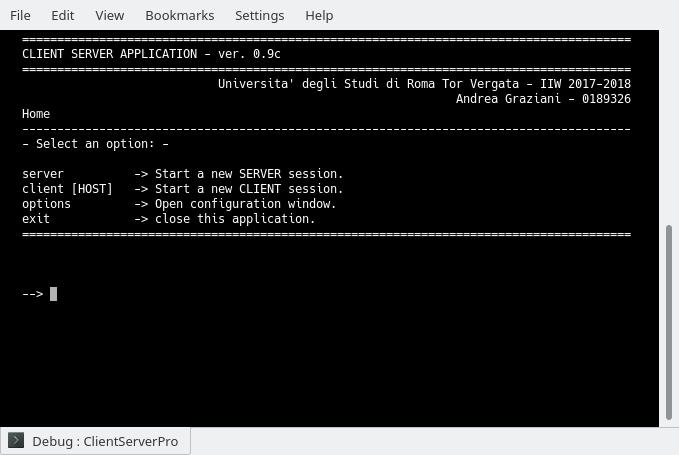
\includegraphics[width=\textwidth]{Home}
\caption{Schermata \textit{Home}.}
\label{fig:home}
\end{figure}

Una volta avviato il programma verrà visualizzata la schermata \textit{Home} riportata in figura \ref{fig:home} attraverso la quale l'utente potrà:
\begin{itemize}
\item Avviare il processo server;
\item Avviare il processo client;
\item Personalizzare le impostazioni;
\item Terminare l'esecuzione dell'applicazione;
\end{itemize}

Come sappiamo, il corretto funzionamento dell'applicazione richiede l'esecuzione contemporanea di un processo server e di uno, o più, processi client. Poiché si è scelto di integrare le funzionalità lato client e server all'interno di uno stesso eseguibile, si è presentata la necessità di implementare un'interfaccia che consenta agli utenti di poter avviare all'occorrenza un processo server o client; questo è lo scopo dell'interfaccia \textit{Home}.

I comandi richiamabili dalla schermata \textit{home} sono quattro:

\begin{description}
\item[\texttt{client [Indirizzo IP processo server]}] Questo comando, seguito dall'indirizzo IP della macchina su cui è in esecuzione il processo server, è utilizzato per avviare, ovviamente, il processo client. Per evitare messaggi di errore, è importante specificare un indirizzo IP valido; da un punto di vista implementativo, il controllo della validità dell'indirizzo IP immesso dell'utente avviene mediante l'esecuzione della funzione \texttt{client\_initialization\_for\_transmission} definita all'interno di \texttt{client\_manager.c} la quale si occupa di allocare e inizializzare una struttura di tipo \texttt{DataNetwork} che verrà poi utilizzata per trasmettere messaggi al server.

\item[\texttt{server}] L'esecuzione di questo comando permette di avviare il processo server il quale una volta avviato rimarrà in attesa di messaggi di richiesta provenienti da uno o più altri processi client. 

\item[\texttt{options}] Il comando permette agli utenti di poter accedere alla schermata \textit{Options} riportata in figura \ref{fig:options} all'interno della quale, attraverso una serie di appositi comandi opportunamente descritti a video, è possibile personalizzare:  

\begin{figure}
\centering
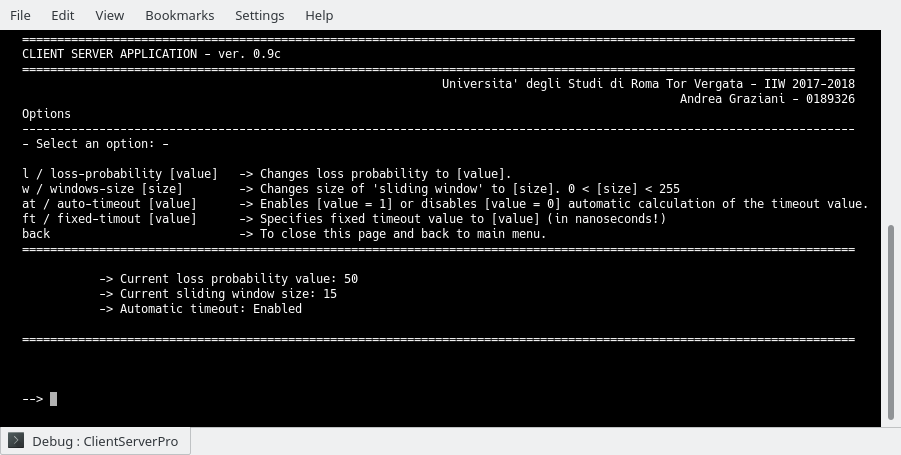
\includegraphics[width=\textwidth]{Options}
\caption{Schermata \textit{Options}.}
\label{fig:options}
\end{figure}

\begin{enumerate}
\item La probabilità di perdita dei messaggi scambiati con il processo server; questo parametro è settato a 0 per impostazione predefinita.
\item La dimensione della finestra di spedizione, settata a 20 per impostazione predefinita.
\item Abilitare/disabilitare il calcolo automatico della durata del timeout. Disabilitando il calcolo automatico, verrà adottato una durata fissa dell'intervallo di timeout; quest'ultimo valore può essere specificato dall'utente. Il calcolo automatico della durata di timeout è abilitato per impostazione predefinita.
\end{enumerate}

Da un punto di vista implementativo, prima dell'invio di un messaggio di richiesta al processo server da parte di un processo client, quest'ultimo legge le impostazioni direttamente dal file system attraverso un apposito file di impostazioni all'interno delle directory principale dell'applicazione. Qualora non venga trovato alcun file di impostazione (perché cancellato o mai creato), l'applicazione provvede a creare un nuovo file popolandolo con le impostazioni di default. 
Quando un processo client deve inoltrare un nuovo messaggio di richiesta al processo server, esso legge le informazioni sulle impostazioni dal file system popolando un'apposita struttura dati denominata \texttt{Settings.c} definita all'interno del file \texttt{Settings.h} e di cui riportiamo il codice in \textit{listing} \ref{code:Settings}; dopo la fase di allocazione e inizializzazione della suddetta struttura, il processo client provvede alla sua serializzazione e copiatura all'interno dei messaggi di richiesta  quindi copiata all'interno dei messaggi di richiesta affinché il processo server sia informato sulle impostazioni dell'utente. La logica di gestione delle impostazioni è descritta all'interno del file \texttt{Settings.c}.

\begin{lstlisting}[frame=lines, caption={Implementazione della struttura \texttt{Settings}}, label={code:Settings}]
typedef struct settings {

	unsigned char sliding_window_size;
	unsigned char loss_probability;
	unsigned char auto_timeout;
	unsigned long fixed_timeout;

} Settings;
\end{lstlisting}
\item[\texttt{exit}] Quest'ultimo comando permette all'utente di poter terminare l'esecuzione del programma.
\end{description}

\newpage
\subsection{Il comando \texttt{list}}\label{sec:list-command}

\begin{figure}
\centering
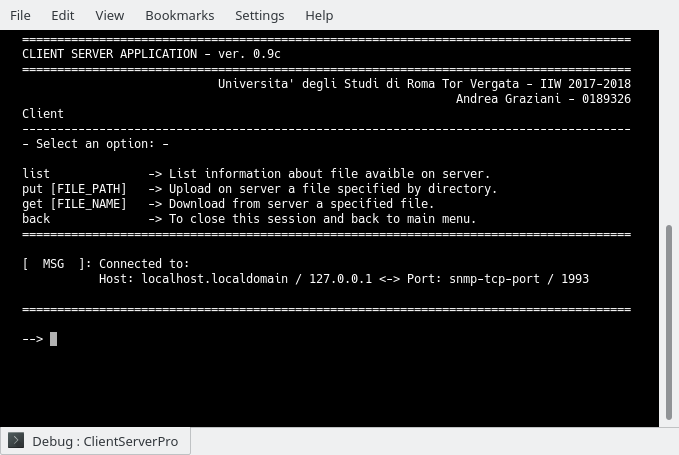
\includegraphics[width=\textwidth]{Client}
\caption{Schermata \textit{Client}.}
\label{fig:Client}
\end{figure}


Per richiedere un elenco dei file disponibili sul server è possibile eseguire il comando \texttt{list} dalla schermata \textit{Client} riportata in figura \ref{fig:Client}, quest'ultima richiamabile dalla schermata \textit{Home} per mezzo del comando \texttt{client}. In caso di successo, verrà riprodotto, in formato tabellare, tutti i nomi, le dimensioni (espresse in byte) e le date di ultimo accesso e modifica dei file disponibili sul server; un esempio dell'output generato dall'esecuzione del comando \texttt{list} è riportata in figura \ref{fig:List}.

\begin{figure}
\centering
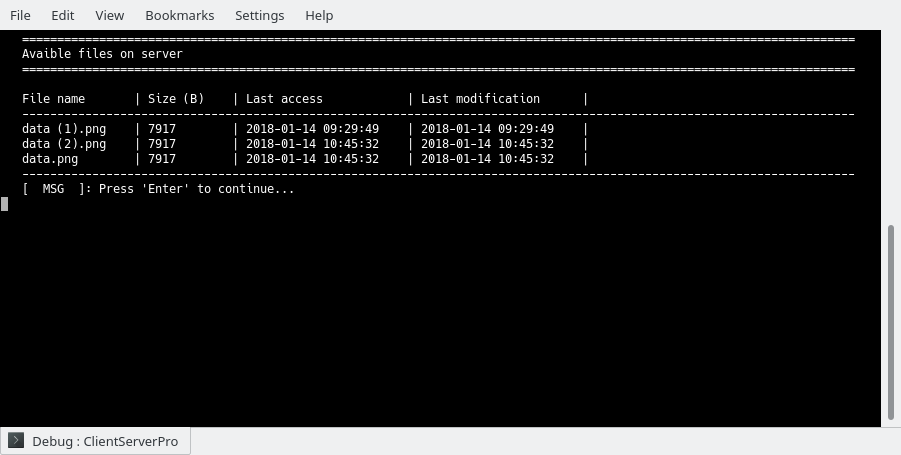
\includegraphics[width=\textwidth]{List}
\caption{Output generato dall'esecuzione del comando \texttt{list}.}
\label{fig:List}
\end{figure}

Da un punto di vista implementativo, dopo la ricezione di un messaggio di richiesta di tipo \texttt{list}, il lavoro svolto dal processo server si divide nelle seguenti fasi:

\begin{description}
\item[Elaborazione directory] Per elaborare correttamente la richiesta di tipo \texttt{list}, il processo server deve innanzitutto stabilire la directory all'interno risiedono i file. Durante questa operazione, attraverso le funzioni definite all'interno del file \texttt{directory\_manager.c}, bisogna innanzitutto stabilire la directory \textit{home} dell'utente che ha avviato il processo server all'interno della quale verranno posizionate tutte le directory necessarie per contenere tutti i file dell'applicazione (file condivisi, meta-dati, file di configurazione ecc.). Una volta nota la directory principale dell'applicazione verrà effettuata la ricerca di quella contenente i file. Il processo server provvede automaticamente alla creazione di tutte le directory necessarie in caso di primo avvio del programma o cancellazione delle directory suddette.  
\item[Lettura e formattazione dati] Una volta stabilita la directory corretta il processo server provvede alla lettura di tutti i file \textit{regolari} presenti in essa. Attraverso la funzione \texttt{get\_file\_information} definita all'interno del file \texttt{FilePropertyList\_struct.c}, il processo server crea, per ogni file elaborato, una struttura di tipo \texttt{FileProperty} all'interno della quale vengono inserite tutte le informazioni di rilievo sui file (nome, dimensione, ecc.). Tutti gli oggetti \texttt{FileProperty} creati verranno inseriti in una lista denominata  \texttt{FilePropertyList}. Queste strutture sono entrambe definite all'interno del file \texttt{FilePropertyList\_struct.h} di cui riportiamo il codice in \textit{listing} \ref{code:FileProperty} e \ref{code:FilePropertyList}.

\begin{lstlisting}[frame=lines, caption={Implementazione della struttura \texttt{FileProperty}}, label={code:FileProperty}]
typedef struct file_property {

	struct stat file_stat;
	char *file_name;

} FileProperty;
\end{lstlisting}

\begin{lstlisting}[frame=lines, caption={Implementazione della struttura \texttt{FileProperty}}, label={code:FilePropertyList}]
typedef struct file_property_list {

	FileProperty *data;

	/* pointer to next node */
	struct file_property_list *next;

} FilePropertyList;
\end{lstlisting}

\item[Serializzazione dati e invio] Per poter inviare al client la struttura dati \texttt{FilePropertyList} precedentemente creata, quest'ultima deve essere innanzitutto serializzarla; dopo la trasmissione, il processo client provvederà a de-serializzare i dati ricevuti e quindi a ricostruire la struttura dati originale per poi elaborarla e visualizzarla all'utente. La responsabilità di dover gestire l'operazione di serializzazione e de-serializzazione è affidata alle funzioni \texttt{FilePropertyList\_serializer} e \texttt{FilePropertyList\_deserializer} entrambe definite e implementate all'interno del file \texttt{FilePropertyList\_struct.c}.
\end{description}

Durante l'esecuzione del processo serve, potrebbe capitare di dover elaborare molte richieste di tipo \texttt{list} obbligando perciò tutti i thread responsabili di gestire le suddette richieste ad eseguire separatemene le stesse operazioni precedentemente descritte; ciò implica un enorme spreco di memoria e potenza computazionale. Pertanto si è preferito implementare un'architettura che preveda l'elaborazione della struttura \texttt{FilePropertyList} una volta soltanto aggiornandola qualora si verificassero operazione di tipo \texttt{put}. Secondo tale implementazione, il processo server provvede alla creazione di un file temporaneo contenente la struttura \texttt{FilePropertyList} già popolata e serializzata in modo tale che tutti i thread responsabili di gestire richieste di tipo \texttt{list} possano inviare direttamente i dati contenuti nel file senza eseguire altre operazioni. La creazione e l'aggiornameto del suddetto file avviene eseguendo la funzione \verb!\__metadata_preload()!; questa funzione viene richiamata sia all'avvio del processo server sia in seguito all'elaborazione di un operazione di tipo \texttt{put}.

\subsection{I comandi \texttt{get} e \texttt{put}}\label{sec:get-put-command}

La trasmissione di dati tra processo client e processo server, avviene attraverso i seguenti comandi richiamabili dalla schermata \textit{Client}:

\begin{description}
\item[\texttt{get [nome file]}] Questo comando permette al client di poter eseguire il donwload di un file disponibile sul server. Affinché l'operazione abbia successo, è importante specificare un nome valido di un file effettivamente disponibile sulla macchina server; in caso contrario il processo server invierà al client un messaggio di errore con la relativa descrizione.
\item[\texttt{put [percorso file]}] Questo comando, seguito da un percorso ad un file valido, permette di eseguire l'upload del suddetto sul server. Se il parametro immesso dell'utente non è valido viene visualizzato un messaggio di errore. Qualora sulla macchina server esistesse già un file avente lo stesso nome del file di cui si intende eseguire l'upload, il processo server rinomina opportunamente il file caricato per evitare conflitti (ad esempio \texttt{nome\_file}, \texttt{nome\_file\_1}, \texttt{nome\_file\_2} ecc.). Al termine dell'operazione, il processo server si occuperà di aggiornare i meta-dati dei file disponibili richiamando la funzione \texttt{\_\_metadata\_preload}.



\end{description}

\newpage
\section{Alcuni esempi di utilizzo dell'applicazione}

\begin{figure}
\centering
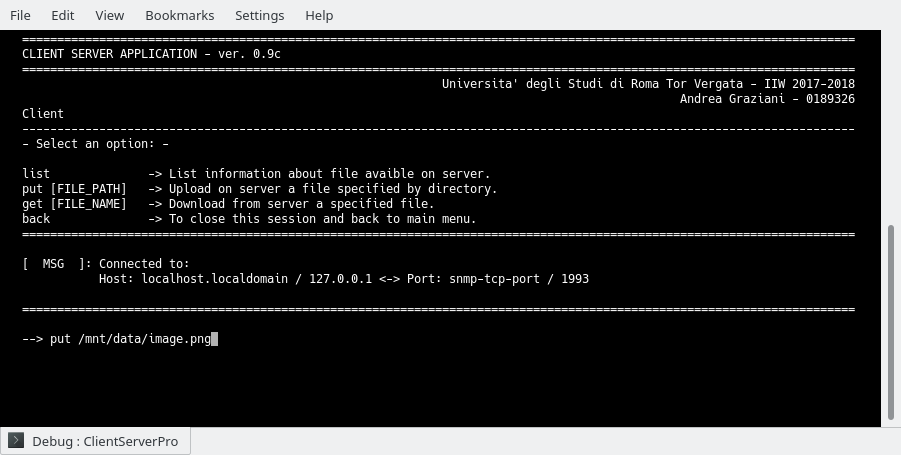
\includegraphics[width=\textwidth]{Example1}
\caption{Esempio di utilizzo del comando \texttt{put}}
\label{fig:example1}
\end{figure}

Giunti a questo punto è doveroso presentare alcuni esempi di utilizzo dell'applicazione. 

Supponiamo di avere in esecuzione il processo server dell'applicazione all'interno della macchina locale. Come abbiamo precedentemente specificato, affinché un client possa interagire con il server, l'utente deve specificare l'indirizzo IP della macchina dove è in esecuzione il processo server. In questo caso digiteremo dalla schermata \textit{Home} il comando \texttt{client localhost}. Qualora digitassimo un indirizzo IP non valido verrà visualizzato un apposito messaggio di errore.

Supponiamo ora di dover eseguire un'operazione di tipo \texttt{put}; in questo scenario supponiamo perciò di voler eseguire l'upload di un file denominato \texttt{image.png} localizzato in \texttt{/mnt/data}.

Come riportato in figura \ref{fig:example1}, dalla schermata \textit{Client} dobbiamo semplicemente digitare il comando \texttt{put /mnt/data/image.png} e dare invio; l'esito dell'operazione ci verrà prontamente comunicato mediante un apposito messaggio.
È molto importante prestare attenzione all'argomento del comando \texttt{put}; la digitazione di un directory o di un file inesistente comporta la visualizzazione di un messaggio di errore. Eventualmente possiamo verificare l'avvenuto trasferimento del file attraverso l'esecuzione del comando \texttt{list}.

Supponiamo ora che un altro client esegua un'operazione di tipo \texttt{put} sullo stesso server caricando un file avente lo stesso nome del file caricato da noi; possiamo simulare quest'eventualità digitando ancora una volta il comando \texttt{put /mnt/data/image.png}. Potete facilmente verificare quanto avvenuto osservando la schermata riportata in figura \ref{fig:example2} ottenuta attraverso l'esecuzione del comando \texttt{list}; come descritto in \ref{sec:get-put-command}, l'applicazione rinomina opportunamente i file per evitare ogni confitto.

\begin{figure}
\centering
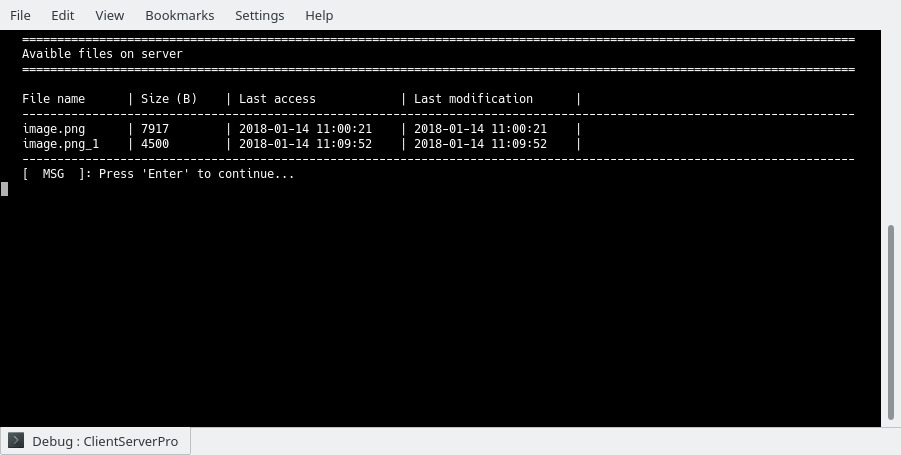
\includegraphics[width=\textwidth,  height=0.25\textheight]{Example2}
\caption{Comportamento dell'applicazione in seguito al caricamento di uno o più file con lo stesso nome}
\label{fig:example2}
\end{figure}

Supponiamo ora di dover eseguire un'operazione di tipo \texttt{get} scaricando dal server il file \textit{image.png}; quello che dobbiamo fare è digitare il comando \texttt{get image.png} dalla schermata \textit{Client} come riportato in figura \ref{fig:example3}. Ricordiamo che il parametro del comando \texttt{get} deve coincidere con il nome di un file presente sul server; se si specifica un nome non valido, l'applicazione restituisce un messaggio di errore. L'esito della suddetta operazione ci verrà prontamente comunicato mediante un apposito messaggio.
Ricordiamo che il file scaricato verrà salvato all'interno della directory \texttt{$\backsim$/ClientServerApplication/client}.

\begin{figure}
\centering
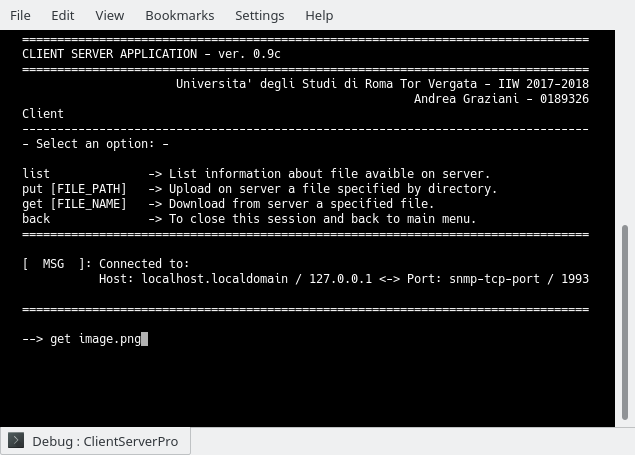
\includegraphics[width=\textwidth, height=0.3\textheight]{Example3}
\caption{Esempio di utilizzo del comando \texttt{get}}
\label{fig:example3}
\end{figure}

\newpage
\section{Descrizione piattaforma software usata per lo sviluppo}

Riportiamo nella tabella \ref{table:akko} i dati della piattaforma utilizzata per lo sviluppo e il test dell'applicazione; è opportuno precisare che tutti i test sono stati eseguiti in locale, ovvero mediante l'esecuzione di un processo server e di un processo client all'interno della stessa macchina.

\begin{table}[H]
\caption{Dati piattaforma software usata per lo sviluppo}\label{table:akko}
\begin{center}
\begin{tabular}{ll}

\toprule

\textbf{IDE} & Eclipse IDE for C/C++ Developers \\
\textbf{Versione IDE} & Oxygen.2 Release (4.7.2), build-id 20171218-0600	\\
\textbf{Sistema operativo} & Arch Linux \\
\textbf{Versione kernel} & v.4.14.13-1-ARCH \\
\textbf{Architettura} & x86\_64 \\

\bottomrule
\end{tabular}
\end{center}
\end{table}

\section{Guida alla compilazione e all'avvio dell'applicazione}

Per eseguire correttamente la compilazione del codice sorgente dell'applicazione occorre:

\begin{enumerate}
\item Estrarre i file contenuti nell'archivio \texttt{ClientServerProject.zip};
\item Eseguire il comando \texttt{make all} all'interno della cartella \texttt{makefile}; l'esecuzione di questo comando genera un eseguibile denominato \texttt{ClientServerProject} all'interno della suddetta cartella.
\end{enumerate}

Dopo la compilazione, per avviare il programma è sufficiente lanciare l'eseguibile \texttt{ClientServerProject} da un qualsiasi emulatore di terminale.
\newpage
\section{Prestazioni}

Riportiamo nella tabella \ref{table:diana} alcuni dati ottenuti sperimentalmente utili per valutare le prestazioni dell'applicazione. 

\begin{savenotes}
\begin{table}[H]
\caption{Analisi sperimentale delle prestazioni dell'applicazione trasferendo un file di dimensione pari a 13,2 $MB$.}\label{table:diana}
\centering
\begin{adjustbox}{width=1.3\textwidth,center=\textwidth}
\small
\begin{tabular}{ccc|ccc|c|cc|c}

\toprule
\multirow{3}{*}{Comando} & 
Dimensione & 
Probabilità & 
\multicolumn{3}{c|}{Pacchetti} & 
Intervallo & 
\multicolumn{2}{c|}{Tempo} &
Esito \\ 
& finestra & di & Dati & Ritrasmessi & Totali \footnote{Include sia pacchetti dati ordinari sia pacchetti di controllo (\texttt{ACK}, \texttt{REQ}, \texttt{FIN} ecc.)} & Timeout & ($s$) & ($ns$) & trasmissione \\
& spedizione & perdita & Elaborati &&&&& & \\		 
 					 
\midrule

\texttt{put}  & 15     & 35\%	& 9236 & 8265 & 17504 & Dinamico & 11  & 575087004 & Riuscita \\
\texttt{put}  & 25     & 35\%	& 9236 & 8126 & 17364 & Dinamico & 21  & 164630756 & Riuscita \\
\texttt{put}  & 35     & 35\%	& 9236 & 8210 & 17449 & Dinamico & 8  & 107812143 & Riuscita \\
\texttt{put}  & 15     & 50\%	& 9236 & 13821 & 23060 & Dinamico & 56  & 833894105 & Riuscita \\
\texttt{put}  & 25     & 50\%	& 9236 & 14157 & 23396 & Dinamico & 70  & 803986995 & Riuscita \\
\texttt{put}  & 35     & 50\%	& 874  & 1385 & 2260 & Dinamico & 46  & 358877914 & Fallita \\
\texttt{put}  & 35     & 50\%	& 9236 & 13909 & 23148 & Dinamico & 47  & 23890293 & Riuscita \\
\texttt{put}  & 35     & 60\%	& 9236 & 19603 & 28842 & Dinamico & 276  & 162591968 & Riuscita \\
\texttt{put}  & 35     & 35\%	& 9236 & 8410 & 17650 &  1 $ms$ & 7  & 109219969 & Riuscita \\
\texttt{put}  & 35     & 35\%	& 9236 & 8170 & 17409 &  10 $ms$ & 61  & 418463705 & Riuscita \\						
\texttt{list}  & 35     & 15\%	& 2 & 1 & 6 &  Dinamico & 0  & 1810316 & Riuscita \\							
\texttt{list}  & 25     & 50\%	& 2 & 3 & 8 &  Dinamico & 0  & 5559479 & Riuscita \\						
\texttt{get}  & 25     & 50\%	& 9236 & 14040 & 23279 &  Dinamico & 77  & 356101859 & Riuscita \\						
\texttt{get}  & 35     & 35\%	& 9236 & 8500 & 17739 & Dinamico & 17  & 269738706 & Riuscita \\
\texttt{get}  & 35     & 0\%	    & 9236 & 0    & 9239 & Dinamico & 0  & 150107979 & Riuscita \\
				
	
				
							

\bottomrule
\end{tabular}
\end{adjustbox}
\end{table}
\end{savenotes}





\listoffigures
\listoftables
\lstlistoflistings

\end{document}













